% A continuación se presentan los anexos del proyecto.\\

% \section{Demostración de la relación entre los parámetros $k_{i}$ para el modelo EDO-WP}

\section{Modelo de optimización por programación lineal entera} 

Con base en lo mencionado en la Sección \ref{linprogmod}, se plantean los conjuntos, las variables, los parámetros y las funciones de objetivo de optimización mediante un ejercicio de optimización lineal que podría prestarse para maximizar ganancias o minimizar emisiones de $[KgCO_{2eq}]$. En esta ocasión se plantea un problema de optimización lineal entera multipropósito, en donde la estimación de ganancia neta que presenta el CA-SENA-POP presenta un conflicto con la reducción de gases de $[KgCO_{2eq}]$, puesto que a mayor producción de estiércol, leche y carne; mayores son las emisiones de estos Gases de Efecto Invernadero (GEI). Así pues, se plantea que:

\subsection{Conjuntos}
\begin{itemize}
\begin{multicols}{2}
    \item $VACAS_{v}$, indexadas por $v$
    \item $DURACIONES_{d}$, indexadas por $d$
    \item $PARTOS_{p}$, indexados por $p$
    \item $DIAS_{t}$, indexados por $t$
    % \item ESCENARIOS, indexados por $s$
\end{multicols}
\end{itemize}
\subsection{Parámetros}

\subsubsection{Emisiones de $[KgCO_{2eq}]$}

\begin{itemize}
    \item Según la ``Nicholas school of environment'' de la Universidad de Duke (\cite{ecoduke}), la producción de un (1) litro de leche representa una generación de  emisiones equivalentes de $Co_{2}$ de aproximadamente $1,39[KgCO_{2eq}/Lt_{leche}]$. Éstas emisiones son denominadas como ``GEIX''.
    \item Según ``Statista.com'', una compañía de estadística comercial a nivel mundial (ver Referencia \cite{statista}), la producción de un (1) kilogramo de peso de ganado dedicado a la producción de leche, representa una generación de  emisiones equivalentes de $Co_{2}$ de aproximadamente $33,3[KgCO_{2eq}/Kg_{carne}]$. Éstas emisiones son denominadas como ``GEIY''.
    \item Según \cite{manure}, la producción de un (1) kilogramo de estiércol representa una generación de  emisiones equivalentes de $Co_{2}$ de aproximadamente $0,0016108[KgCO_{2eq}/Kg_{estiercol}]$. Éstas emisiones son denominadas como ``GEIZ''.
\end{itemize}
% \subsubsection{Costos de producción}
% \begin{itemize}
%     \item Hasta donde sé el sena no me ha dado estos datos, probablemente no los tienen a la mano, entonces mejor no lo considero
% \end{itemize}
% \pagebreak

\subsubsection{Precios de venta}

\begin{itemize}
    \item Según el CA-SENA-POP (ver Referencia \cite{casena}), el precio  de venta promedio de un (1) kilogramo de carne de res hembra (PVY) es de aproximadamente $7100[\$Pesos/Kg_{peso}]$. 
    \item Según el CA-SENA-POP (ver Referencia \cite{casena}), el precio de venta de un (1) kilogramo de leche cruda sin análisis de proteína y grasas (PVX) es de aproximadamente $1350[\frac{\$Pesos}{Kg_{leche-cruda}}]$.
\end{itemize}

\subsubsection{Producción}

\begin{itemize}
    \item Según los registros proporcionados de manera física y digital del CA-SENA-POP (ver Referencia \cite{casena}), las producciones mínimas de leche pueden representarse como un parámetro $PMINX_{vp}$ en [$Kg_{leche}$/$Vaca_{v}Parto_{p}$]
    \item Según los registros proporcionados de manera física y digital del CA-SENA-POP (ver Referencia \cite{casena}), las producciones mínimas de carne pueden representarse como un parámetro $PMINY_{vp}$ en [$Kg_{carne}$/$Vaca_{v}Parto_{p}$]
    \item Según los registros proporcionados de manera física y digital del CA-SENA-POP (ver Referencia \cite{casena}), las producciones mínimas de estiércol pueden representarse como un parámetro $PMINZ_{vp}$ en [$Kg_{estiercol}$/$Vaca_{v}Parto_{p}$]
    \item Según los registros proporcionados de manera física y digital del CA-SENA-POP (ver Referencia \cite{casena}), las producciones máximas de leche pueden representarse como un parámetro $PMAXX_{vp}$ en [$Kg_{leche}$/$Vaca_{v}Parto_{p}$]
     \item Según los registros proporcionados de manera física y digital del CA-SENA-POP (ver Referencia \cite{casena}), las producciones máximas de carne pueden representarse como un parámetro $PMAXY_{vp}$ en [$Kg_{carne}$/$Vaca_{v}Parto_{p}$]
      \item Según los registros proporcionados de manera física y digital del CA-SENA-POP (ver Referencia \cite{casena}), las producciones máximas de leche pueden representarse como un parámetro $PMAXZ_{vp}$ en [$Kg_{estiercol}$/$Vaca_{v}Parto_{p}$]
    % \item Según el CA-SENA-POP (\cite{casena}), el precio de venta de un (1) kilogramo de leche cruda (PVKGLEC) es de aproximadamente $1350[\frac{\$Pesos}{Kg_{leche-cruda}}]$.
\end{itemize}

\subsection{Variables}
\begin{itemize}
    \item \textbf{$\mathcal{X}_{vpdts}$} $\longrightarrow$ Cantidad de leche producida por una vaca $v$ en un grupo de parto $p$ que tiene una duración de lactancia aproximada $d$ en un día $t$; en [$Kg_{Leche}$]. $\left(\mathcal{X}_{vpdts}\geq 0 \right)$.
    % \item \textbf{$\mathcal{X}_{vpdts}$}, Cantidad de leche producida por una vaca $v$ en un grupo de parto $p$ que tiene una duración de lactancia aproximada $d$ en un día $t$ en un escenario $s$; en [$Kg_{Leche}$].
    % \begin{equation*}
    %     \mathcal{X}_{ijdts}
    % \end{equation*}
    \item \textbf{$\mathcal{Y}_{vpdts}$}$\longrightarrow$ Cantidad de carne producido por una vaca $v$ en un grupo de parto $p$ que tiene una duración de lactancia aproximada $d$ en un día $t$; en [$Kg_{Carne}$].  $\left(\mathcal{Y}_{vpdts}\geq 0 \right)$.
    % \item \textbf{$\mathcal{Y}_{vpdts}$}, Cantidad de carne producido por una vaca $v$ en un grupo de parto $p$ que tiene una duración de lactancia aproximada $d$ en un día $t$ en un escenario $s$; en [$Kg_{Carne}$].
    % \begin{equation*}
    %     \mathcal{Y}_{ijdts}
    % \end{equation*}

    \item \textbf{$\mathcal{Z}_{vpdts}$}$\longrightarrow$ Cantidad de estiércol producido por una vaca $v$ en un grupo de parto $p$ que tiene una duración de lactancia aproximada $d$ en un día $t$; en [$Kg_{Estiercol}$].  $\left(\mathcal{Z}_{vpdts}\geq 0 \right)$.
    % \item \textbf{$\mathcal{Z}_{vpdts}$}, Cantidad de estiércol producido por una vaca $v$ en un grupo de parto $p$ que tiene una duración de lactancia aproximada $d$ en un día $t$ en un escenario $s$; en [$Kg_{Estiercol}$].
\end{itemize}

\subsection{Funciones objetivo}

\subsubsection{Maximizar ganancias}

Si el planteamiento del modelo se enfoca en maximizar las ganancias sin importar el posible impacto ecológico, la función objetivo del modelo lineal estará representada por la ecuación \ref{ecutil}. Se debe mencionar que para este análisis no se tiene conocimiento de los costos operacionales del CA-SENA-POP, por lo que son considerados como nulos para este caso. En una situación donde se tenga conocimiento de estos valores económicos, basta con substraer el costo operacional asociado a cada lactancia monitoreada que puede ser considerado como un parámetro $COPER_{vpdt}$ (si el costo es diario durante toda la lactancia) ó $COPER_{vp}$ (si el costo es total, resultado de todo el periodo de lactancia).
\begin{equation}\label{ecutil}
\begin{split}
    Max(UTILIDADES) =\left(PVX\sum_{v,p,d,t}\mathcal{X}_{vpdt}\right) + \left(PVY\sum_{v,p,d,t}\mathcal{Y}_{vpdt} \right) - \sum_{v,p,d,t}COPER_{vpdt}
\end{split}
\end{equation}

\subsubsection{Minimizar emisiones de gases de efecto invernadero GEI.}

Si nos centramos únicamente en plantear el modelo para minimizar las emisiones de GEI sin tener en consideración las posibles repercusiones financieras que estas producciones puedan representar, se tiene un modelo lineal cuya función objetivo estará representada por la siguiente ecuación:
\begin{equation}\label{ecemis}
\begin{split}
    Min(EMISIONES) =\left( GEIX\sum_{v,p,d,t}\mathcal{X}_{vpdt}\right) + \left(GEIY\sum_{v,p,d,t}\mathcal{Y}_{vpdt}\right) + \left(GEIZ\sum_{v,p,d,t}\mathcal{Z}_{vpdt} \right)
\end{split}
\end{equation}

% \subsubsection{Multi-objetivo: Ganancia máxima y emisiones mínimas}

\subsection{Restricciones}

\subsubsection{Producción mínima}

\begin{itemize}
\begin{multicols}{2}
    \item \textbf{$\mathcal{X}_{vpdts}\geq PMINX_{vp}$} $\longrightarrow \forall v,p $
    \item \textbf{$\mathcal{Z}_{vpdts}\geq PMINZ_{vp}$} $\longrightarrow \forall v,p $
    \item \textbf{$\mathcal{Y}_{vpdts}\geq PMINY_{vp}$} $\longrightarrow \forall v,p $
    \item $PMINX_{vp}$, $PMINY_{vp}$, $PMINZ_{vp}$, $\geq 0$
    
\end{multicols}
\end{itemize}

\subsubsection{Producción máxima}

\begin{itemize}
\begin{multicols}{2}
    \item \textbf{$\mathcal{X}_{vpdts}\leq PMAXX_{vp}$} $\longrightarrow \forall v,p $
    \item \textbf{$\mathcal{Z}_{vpdts}\leq PMAXZ_{vp}$} $\longrightarrow \forall v,p$
    \item \textbf{$\mathcal{Y}_{vpdts}\leq PMAXY_{vp}$} $\longrightarrow \forall v,p$
    \item $PMAXX_{vp}$, $PMAXY_{vp}$, $PMAXZ_{vp}$, $\geq 0$
    
\end{multicols}
\end{itemize}
% \pagebreak

\section{Tabla \ref{tab:allparams} - Parámetros de ajuste para cada método usado.}
% [1-49]  --- INCLUYE los "parametros" sacados de los registros
% \begin{sidewaystable}%[H]
% % \begin{table}
% \centering
% \caption{Resumen de los parámetros de ajuste para cada método usado y su respectivo MSE.} \label{tab:allparams}
% \resizebox{0.95\textwidth}{!}{\begin{tabular}{|cc|c|ccc|cccc|cccc|ccccc|ccccc|}
 
%     \hline
%      \cellcolor[HTML]{FFD9AC} &  \cellcolor[HTML]{FFD9AC} & \cellcolor[HTML]{FFD9AC}  & \cellcolor[HTML]{FFD9AC} & \cellcolor[HTML]{FFD9AC}REGISTROS & \cellcolor[HTML]{FFD9AC} & \cellcolor[HTML]{FFD9AC} & \cellcolor[HTML]{FFD9AC} LMA & \cellcolor[HTML]{FFD9AC} & \cellcolor[HTML]{FFD9AC} & \cellcolor[HTML]{FFD9AC} & \cellcolor[HTML]{FFD9AC} ``Super Vaca''  & \cellcolor[HTML]{FFD9AC} &\cellcolor[HTML]{FFD9AC} &\cellcolor[HTML]{FFD9AC}  &\cellcolor[HTML]{FFD9AC} & \cellcolor[HTML]{FFD9AC} NLFEA & \cellcolor[HTML]{FFD9AC} & \cellcolor[HTML]{FFD9AC} & \cellcolor[HTML]{FFD9AC} & \cellcolor[HTML]{FFD9AC} & \cellcolor[HTML]{FFD9AC} NLREA & \cellcolor[HTML]{FFD9AC}  & \cellcolor[HTML]{FFD9AC} \\
%      \cellcolor[HTML]{FFD9AC}PARTO $P\#_{i}$ & \cellcolor[HTML]{FFD9AC}N & \cellcolor[HTML]{FFD9AC}PARS & \cellcolor[HTML]{FFD9AC}$\alpha$ & \cellcolor[HTML]{FFD9AC}$\beta$ & \cellcolor[HTML]{FFD9AC}$\gamma$ & \cellcolor[HTML]{FFD9AC}$\alpha$ & \cellcolor[HTML]{FFD9AC}$\beta$ & \cellcolor[HTML]{FFD9AC}$\gamma$ & \cellcolor[HTML]{FFD9AC}MSE-I & \cellcolor[HTML]{FFD9AC}$\alpha$ & \cellcolor[HTML]{FFD9AC}$\beta$ & \cellcolor[HTML]{FFD9AC}$\gamma$ & \cellcolor[HTML]{FFD9AC}MSE-G & \cellcolor[HTML]{FFD9AC}$\alpha$ & \cellcolor[HTML]{FFD9AC}$\beta$ & \cellcolor[HTML]{FFD9AC}$\gamma$ & \cellcolor[HTML]{FFD9AC}MSE-I & \cellcolor[HTML]{FFD9AC}MSE-G & \cellcolor[HTML]{FFD9AC}$\alpha$ & \cellcolor[HTML]{FFD9AC}$\beta$ &\cellcolor[HTML]{FFD9AC} $\gamma$ & \cellcolor[HTML]{FFD9AC}MSE-I & \cellcolor[HTML]{FFD9AC}MSE-G\\
%      \cellcolor[HTML]{FFD9AC} & \cellcolor[HTML]{FFD9AC} & \cellcolor[HTML]{FFD9AC}VACA &\cellcolor[HTML]{FFD9AC} &\cellcolor[HTML]{FFD9AC} &\cellcolor[HTML]{FFD9AC} &\cellcolor[HTML]{FFD9AC} &\cellcolor[HTML]{FFD9AC} &\cellcolor[HTML]{FFD9AC} &\cellcolor[HTML]{FFD9AC} & \cellcolor[HTML]{FFD9AC}&\cellcolor[HTML]{FFD9AC} & \cellcolor[HTML]{FFD9AC}& \cellcolor[HTML]{FFD9AC}&\cellcolor[HTML]{FFD9AC} &\cellcolor[HTML]{FFD9AC} &\cellcolor[HTML]{FFD9AC} &\cellcolor[HTML]{FFD9AC} &\cellcolor[HTML]{FFD9AC} &\cellcolor[HTML]{FFD9AC} &\cellcolor[HTML]{FFD9AC} &\cellcolor[HTML]{FFD9AC} & \cellcolor[HTML]{FFD9AC} & \cellcolor[HTML]{FFD9AC} \\
%      \hline
%      \cellcolor[HTML]{343434} & \cellcolor[HTML]{343434} & \cellcolor[HTML]{656565}\color[HTML]{FFFFFF}ACER & 15.500 & 0.045 & 0.007 & 9.602& 0.153& 0.004& 3.930 & & & & &9.612 & 0.147 & 0.003 & 3.848 &  & 10.098 & 0.131 & 0.003 & 3.921 & \\
%      \cellcolor[HTML]{343434} \color[HTML]{FFFFFF}$P\#_{1}$ & \cellcolor[HTML]{343434} \color[HTML]{FFFFFF}299 & \cellcolor[HTML]{656565}\color[HTML]{FFFFFF}SOL & 7.000 & 0.210 & 0.008 & 7.405 & 0.119 & 0.003 & 4.706 & 8.273& 0.125 & 0.003 & 6.824 & 8.295 & 0.079 & 0.002& 4.682 & 4.486 & 6.833 & 0.131 & 0.003 & 4.750 & 4.485\\
%      \cellcolor[HTML]{343434}& \cellcolor[HTML]{343434}& \cellcolor[HTML]{656565}\color[HTML]{FFFFFF}LUN & 5.400 & 0.317 & 0.006 & 7.067 & 0.136 & 0.003 & 4.775 & & & & & 6.986 & 0.140 & 0.003 & 4.7829 &  & 7.375 & 0.131 & 0.003 & 5.036 & \\
%      \hline
%      \cellcolor[HTML]{3241CB}& \cellcolor[HTML]{3241CB}& \cellcolor[HTML]{BDFFFC}DIAN & 21.000 & 0.080 & 0.005 & 15.930 & 0.114 & 0.004 & 12.523 & & & & & 16.220 & 0.107 & 0.004 & 11.949 &  & 16.154 & 0.109 & 0.004 & 11.955 & \\
%      \cellcolor[HTML]{3241CB}& \cellcolor[HTML]{3241CB}& \cellcolor[HTML]{BDFFFC}GINA & 20.400 & 0.168 & 0.009 & 11.950 & 0.251 & 0.007& 3.292 & & & & & 16.059 & 0.149 & 0.006 & 3.230 &  & 15.553 & 0.158 & 0.006 & 3.248 & \\
%      \cellcolor[HTML]{3241CB}& \cellcolor[HTML]{3241CB}& \cellcolor[HTML]{BDFFFC}JUAN & 9.400 & 0.126 & 0.010 & 4.103 & 0.317 & 0.008 & 8.128 & & & & & 4.384 & 0.282 & 0.007 & 8.074 &  & 5.119 & 0.233 & 0.007 & 8.112 & \\
%      \cellcolor[HTML]{3241CB}\color[HTML]{FFFFFF}$P\#_{2}$ & \cellcolor[HTML]{3241CB}\color[HTML]{FFFFFF}288 & \cellcolor[HTML]{BDFFFC}LUCI & 19.000 & 0.028 & 0.005 & 13.394 & 0.167 & 0.007 & 4.967 & 12.210 & 0.154 & 0.053 & 17.828 & 13.801 & 0.147 & 0.006 & 4.985 & 8.455 & 13.127 & 0.160 & 0.006 & 4.987 & 8.448\\
%      \cellcolor[HTML]{3241CB}& \cellcolor[HTML]{3241CB}& \cellcolor[HTML]{BDFFFC}PAC & 18.600 & 0.069 & 0.004 & 20.167& -0.036& 0.002 & 9.489 & & & & &19.752 &-0.027 &0.002 & 9.346 &  & 18.765 &-0.010 &0.002 & 9.363 & \\
%      \cellcolor[HTML]{3241CB}& \cellcolor[HTML]{3241CB}& \cellcolor[HTML]{BDFFFC}SOL & 16.800 & 0.078 & 0.008 &10.138 &0.220 &0.007 & 16.013 & & & & & 9.374 & 0.238 & 0.007 & 15.887 &  & 9.673 & 0.227 & 0.007 & 15.890 & \\
%      \cellcolor[HTML]{3241CB}& \cellcolor[HTML]{3241CB}& \cellcolor[HTML]{BDFFFC}VIV & 15.400 & 0.094 & 0.008 &6.794 &0.339 &0.007 & 5.043 & & & & & 7.847 &0.290 &0.007 & 5.017 &  & 8.830 &0.256 &0.006 & 5.034 & \\
%      \hline
%     \cellcolor[HTML]{32CB00} & \cellcolor[HTML]{32CB00}& \cellcolor[HTML]{AAFF85}FER & 21.000 & 0.101 & 0.006 & 19.729 & 0.064 & 0.003 & 9.721 & & & & & 20.217 & 0.052 & 0.003 & 9.698 &  & 19.466 & 0.067 & 0.003 & 9.704 & \\
%      \cellcolor[HTML]{32CB00}& \cellcolor[HTML]{32CB00}& \cellcolor[HTML]{AAFF85}GPA & 22.000 & 0.099 & 0.005 & 15.206 & 0.148 & 0.004 & 11.415 & & & & & 15.638 & 0.132 & 0.004 & 11.420 &  & 15.506 & 0.136 & 0.004 & 11.422 & \\
%      \cellcolor[HTML]{32CB00}& \cellcolor[HTML]{32CB00}& \cellcolor[HTML]{AAFF85}JUAN & 11.000 & 0.208 & 0.007 & 9.445 & 0.203 & 0.004 & 4.692 & & & & & 9.485 & 0.202 & 0.004 & 4.712 &  & 9.907 & 0.190 & 0.004 & 4.713 & \\
%      \cellcolor[HTML]{32CB00}$P\#_{3}$ & \cellcolor[HTML]{32CB00}309 & \cellcolor[HTML]{AAFF85}LETI & 16.200 & 0.116 & 0.008 & 15.388 & 0.098 & 0.004 & 22.970 & 13.711 & 0.146 & 0.004 & 21.470 & 16.645 & 0.069 & 0.003 & 22.965 & 12.762 & 16.298 & 0.073 & 0.004 & 22.993 & 12.747\\
%      \cellcolor[HTML]{32CB00}& \cellcolor[HTML]{32CB00}& \cellcolor[HTML]{AAFF85}MART & 10.800 & 0.283 & 0.007 & 6.613& 0.392& 0.006 & 17.059 & & & & &6.516 &0.396 &0.006 & 17.039 &  & 7.084 &0.371 &0.006 & 17.076 & \\
%      \cellcolor[HTML]{32CB00}& \cellcolor[HTML]{32CB00}& \cellcolor[HTML]{AAFF85}MOR & 22.000 & 0.157 & 0.009 &19.921 &0.108 &0.004 & 11.914 & & & & &20.858 &0.092 &0.004 & 11.871 &  & 20.353 &0.096 &0.004 & 11.899 & \\
%      \cellcolor[HTML]{32CB00}&\cellcolor[HTML]{32CB00} & \cellcolor[HTML]{AAFF85}SOL & 16.000 & 0.064 & 0.006 &12.511 &0.058 &0.003 & 10.689 & & & & & 12.452 &0.059 &0.003 & 10.670 &  & 12.282 &0.064 &0.003 & 10.678 & \\
%      \hline
%      \cellcolor[HTML]{FFFE65}& \cellcolor[HTML]{FFFE65}& \cellcolor[HTML]{FFFFC7}CENT & 6.600 & 0.211 & 0.008 & 4.030 & 0.375 & 0.005 & 12.678 & & & & & 4.908 & 0.314 & 0.004 & 12.612 &  & 5.959 & 0.259 & 0.004 & 12.622 & \\
%      \cellcolor[HTML]{FFFE65}& \cellcolor[HTML]{FFFE65}& \cellcolor[HTML]{FFFFC7}DIAN & 11.400 & 0.106 & 0.005 & 10.448 & 0.073 & 0.003 & 11.537 & & & & & 10.658 & 0.067 & 0.002 & 11.424 &  & 9.965 & 0.090 & 0.003 & 11.436 & \\
%      \cellcolor[HTML]{FFFE65}&\cellcolor[HTML]{FFFE65} & \cellcolor[HTML]{FFFFC7}LETI & 15.000 & 0.089 & 0.007 & 11.952 & 0.073 & 0.003 & 9.446 & & & & & 12.857 & 0.043 & 0.003 & 9.415 &  & 11.721 & 0.073 & 0.030 & 9.429 & \\
%      \cellcolor[HTML]{FFFE65}$P\#_{4}$ & \cellcolor[HTML]{FFFE65}274 & \cellcolor[HTML]{FFFFC7}MOR & 15.300 & 0.077 & 0.004 & 12.251 & 0.124 & 0.005 & 5.594 & 9.530 & 0.144 & 0.004 & 12.435 & 13.101 & 0.095 & 0.004 & 5.462 & 8.78 & 12.301 & 0.115 & 0.004 & 5.514 & 8.773 \\
%      \cellcolor[HTML]{FFFE65}& \cellcolor[HTML]{FFFE65}& \cellcolor[HTML]{FFFFC7}MUC & 16.200 & 0.088 & 0.006 & 12.259 & 0.182 & 0.007 & 9.440 & & & & & 13.138 & 0.155 & 0.006 & 9.398 &  & 12.708 & 0.164 & 0.006 & 9.425 & \\
%      \cellcolor[HTML]{FFFE65}& \cellcolor[HTML]{FFFE65}& \cellcolor[HTML]{FFFFC7}SOR & 4.800 & 0.311 & 0.010 & 5.386 & 0.262 & 0.007 & 9.044 & & & & & 5.404 & 0.263 & 0.007 & 8.943 &  & 6.297 & 0.209 & 0.006 & 8.949 & \\
%      \cellcolor[HTML]{FFFE65}& \cellcolor[HTML]{FFFE65}& \cellcolor[HTML]{FFFFC7}VIV & 12.200 & 0.138 & 0.005 &7.032 &0.210 &0.004 & 3.401 & & & & & 6.831 &0.208 &0.004 & 3.403 &  & 7.370 &0.186 &0.004 & 3.442 & \\
%      \hline
%      \cellcolor[HTML]{D34444}$P\#_{5}$ & \cellcolor[HTML]{D34444}298 & \cellcolor[HTML]{FFCCC9}GPA & 11.000 & 0.169 & 0.009 & 1.619 & 0.688 & 0.009 & 9.345 & 4.246 & 0.425 & 0.007 & 11.388 & 1.531 & 0.705 & 0.009 & 9.270 & 9.440 & 1.670 & 0.679 & 0.009 & 9.278 & 9.440\\
%      \cellcolor[HTML]{D34444}& \cellcolor[HTML]{D34444}& \cellcolor[HTML]{FFCCC9}ANDRE & 8.600 & 0.258 & 0.008 & 9.473 & 0.213 & 0.005 & 9.553 & & & & & 9.881 & 0.193 & 0.004 & 9.409 &  & 9.371 & 0.210 & 0.005 & 9.418 & \\
%      \hline
%      \cellcolor[HTML]{6665CD}$P\#_{6}$ & \cellcolor[HTML]{6665CD}162 & \cellcolor[HTML]{CBCEFB}GPA & 13.000 & 0.173 & 0.005 & 14.928 & 0.149 & 0.004 & 4.801 & 15.118 & 0.136 & 0.004 & 4.869 & 14.977 & 0.146 & 0.004 & 4.802 & 4.652 & 15.118 & 0.136 & 0.004 & 4.995 & 4.648\\
%      \cellcolor[HTML]{6665CD}&\cellcolor[HTML]{6665CD} & \cellcolor[HTML]{CBCEFB}ANDRE & 19.20 & 0.077 & 0.007 & 15.437 & 0.118 & 0.004 & 4.482 & & & & & 15.247 & 0.125 & 0.004 & 4.436 &  & 15.105 & 0.136 & 0.004 & 4.624 & \\
%      \hline
%  \end{tabular}}
% % \end{table}
% \end{sidewaystable}





% [55 - 105]--- no tiene los "parametros" sacados de los registros

\begin{sidewaystable}%[H]
% \begin{table}
\centering
\caption{Resumen de los parámetros de ajuste para cada método usado y su respectivo MSE.} \label{tab:allparams}

\resizebox{0.95\textwidth}{!}{\begin{tabular}{|cc|c|cccc|cccc|ccccc|ccccc|}
 
    \hline
     \cellcolor[HTML]{FFD9AC} &  \cellcolor[HTML]{FFD9AC} & \cellcolor[HTML]{FFD9AC}  & \cellcolor[HTML]{FFD9AC} & \cellcolor[HTML]{FFD9AC} LMA & \cellcolor[HTML]{FFD9AC} & \cellcolor[HTML]{FFD9AC} & \cellcolor[HTML]{FFD9AC} & \cellcolor[HTML]{FFD9AC} ``Super Vaca''  & \cellcolor[HTML]{FFD9AC} &\cellcolor[HTML]{FFD9AC} &\cellcolor[HTML]{FFD9AC}  &\cellcolor[HTML]{FFD9AC} & \cellcolor[HTML]{FFD9AC} NLFEA & \cellcolor[HTML]{FFD9AC} & \cellcolor[HTML]{FFD9AC} & \cellcolor[HTML]{FFD9AC} & \cellcolor[HTML]{FFD9AC} & \cellcolor[HTML]{FFD9AC} NLREA & \cellcolor[HTML]{FFD9AC}  & \cellcolor[HTML]{FFD9AC} \\
     \cellcolor[HTML]{FFD9AC}PARTO $P\#_{i}$ & \cellcolor[HTML]{FFD9AC}N & \cellcolor[HTML]{FFD9AC}PARS & \cellcolor[HTML]{FFD9AC}$\alpha$ & \cellcolor[HTML]{FFD9AC}$\beta$ & \cellcolor[HTML]{FFD9AC}$\gamma$ & \cellcolor[HTML]{FFD9AC}MSE-I & \cellcolor[HTML]{FFD9AC}$\alpha$ & \cellcolor[HTML]{FFD9AC}$\beta$ & \cellcolor[HTML]{FFD9AC}$\gamma$ & \cellcolor[HTML]{FFD9AC}MSE-G & \cellcolor[HTML]{FFD9AC}$\alpha$ & \cellcolor[HTML]{FFD9AC}$\beta$ & \cellcolor[HTML]{FFD9AC}$\gamma$ & \cellcolor[HTML]{FFD9AC}MSE-I & \cellcolor[HTML]{FFD9AC}MSE-G & \cellcolor[HTML]{FFD9AC}$\alpha$ & \cellcolor[HTML]{FFD9AC}$\beta$ &\cellcolor[HTML]{FFD9AC} $\gamma$ & \cellcolor[HTML]{FFD9AC}MSE-I & \cellcolor[HTML]{FFD9AC}MSE-G\\
     \cellcolor[HTML]{FFD9AC} & \cellcolor[HTML]{FFD9AC} & \cellcolor[HTML]{FFD9AC}VACA &\cellcolor[HTML]{FFD9AC} &\cellcolor[HTML]{FFD9AC} &\cellcolor[HTML]{FFD9AC} &\cellcolor[HTML]{FFD9AC} & \cellcolor[HTML]{FFD9AC}&\cellcolor[HTML]{FFD9AC} & \cellcolor[HTML]{FFD9AC}& \cellcolor[HTML]{FFD9AC}&\cellcolor[HTML]{FFD9AC} &\cellcolor[HTML]{FFD9AC} &\cellcolor[HTML]{FFD9AC} &\cellcolor[HTML]{FFD9AC} &\cellcolor[HTML]{FFD9AC} &\cellcolor[HTML]{FFD9AC} &\cellcolor[HTML]{FFD9AC} &\cellcolor[HTML]{FFD9AC} & \cellcolor[HTML]{FFD9AC} & \cellcolor[HTML]{FFD9AC} \\
     \hline
     \cellcolor[HTML]{343434} & \cellcolor[HTML]{343434} & \cellcolor[HTML]{656565}\color[HTML]{FFFFFF}ACER & 9.602& 0.153& 0.004& 3.930 & & & & &9.612 & 0.147 & 0.003 & 3.848 &  & 10.098 & 0.131 & 0.003 & 3.921 & \\
     \cellcolor[HTML]{343434} \color[HTML]{FFFFFF}$P\#_{1}$ & \cellcolor[HTML]{343434} \color[HTML]{FFFFFF}299 & \cellcolor[HTML]{656565}\color[HTML]{FFFFFF}SOL & 7.405 & 0.119 & 0.003 & 4.706 & 8.273& 0.125 & 0.003 & 6.824 & 8.295 & 0.079 & 0.002& 4.682 & 4.486 & 6.833 & 0.131 & 0.003 & 4.750 & 4.485\\
     \cellcolor[HTML]{343434}& \cellcolor[HTML]{343434}& \cellcolor[HTML]{656565}\color[HTML]{FFFFFF}LUN & 7.067 & 0.136 & 0.003 & 4.775 & & & & & 6.986 & 0.140 & 0.003 & 4.7829 &  & 7.375 & 0.131 & 0.003 & 5.036 & \\
     \hline
     \cellcolor[HTML]{3241CB}& \cellcolor[HTML]{3241CB}& \cellcolor[HTML]{BDFFFC}DIAN & 15.930 & 0.114 & 0.004 & 12.523 & & & & & 16.220 & 0.107 & 0.004 & 11.949 &  & 16.154 & 0.109 & 0.004 & 11.955 & \\
     \cellcolor[HTML]{3241CB}& \cellcolor[HTML]{3241CB}& \cellcolor[HTML]{BDFFFC}GINA & 11.950 & 0.251 & 0.007& 3.292 & & & & & 16.059 & 0.149 & 0.006 & 3.230 &  & 15.553 & 0.158 & 0.006 & 3.248 & \\
     \cellcolor[HTML]{3241CB}& \cellcolor[HTML]{3241CB}& \cellcolor[HTML]{BDFFFC}JUAN & 4.103 & 0.317 & 0.008 & 8.128 & & & & & 4.384 & 0.282 & 0.007 & 8.074 &  & 5.119 & 0.233 & 0.007 & 8.112 & \\
     \cellcolor[HTML]{3241CB}\color[HTML]{FFFFFF}$P\#_{2}$ & \cellcolor[HTML]{3241CB}\color[HTML]{FFFFFF}288 & \cellcolor[HTML]{BDFFFC}LUCI & 13.394 & 0.167 & 0.007 & 4.967 & 12.210 & 0.154 & 0.053 & 17.828 & 13.801 & 0.147 & 0.006 & 4.985 & 8.455 & 13.127 & 0.160 & 0.006 & 4.987 & 8.448\\
     \cellcolor[HTML]{3241CB}& \cellcolor[HTML]{3241CB}& \cellcolor[HTML]{BDFFFC}PAC & 20.167& -0.036& 0.002 & 9.489 & & & & &19.752 &-0.027 &0.002 & 9.346 &  & 18.765 &-0.010 &0.002 & 9.363 & \\
     \cellcolor[HTML]{3241CB}& \cellcolor[HTML]{3241CB}& \cellcolor[HTML]{BDFFFC}SOL &10.138 &0.220 &0.007 & 16.013 & & & & & 9.374 & 0.238 & 0.007 & 15.887 &  & 9.673 & 0.227 & 0.007 & 15.890 & \\
     \cellcolor[HTML]{3241CB}& \cellcolor[HTML]{3241CB}& \cellcolor[HTML]{BDFFFC}VIV &6.794 &0.339 &0.007 & 5.043 & & & & & 7.847 &0.290 &0.007 & 5.017 &  & 8.830 &0.256 &0.006 & 5.034 & \\
     \hline
    \cellcolor[HTML]{32CB00} & \cellcolor[HTML]{32CB00}& \cellcolor[HTML]{AAFF85}FER & 19.729 & 0.064 & 0.003 & 9.721 & & & & & 20.217 & 0.052 & 0.003 & 9.698 &  & 19.466 & 0.067 & 0.003 & 9.704 & \\
     \cellcolor[HTML]{32CB00}& \cellcolor[HTML]{32CB00}& \cellcolor[HTML]{AAFF85}GPA & 15.206 & 0.148 & 0.004 & 11.415 & & & & & 15.638 & 0.132 & 0.004 & 11.420 &  & 15.506 & 0.136 & 0.004 & 11.422 & \\
     \cellcolor[HTML]{32CB00}& \cellcolor[HTML]{32CB00}& \cellcolor[HTML]{AAFF85}JUAN & 9.445 & 0.203 & 0.004 & 4.692 & & & & & 9.485 & 0.202 & 0.004 & 4.712 &  & 9.907 & 0.190 & 0.004 & 4.713 & \\
     \cellcolor[HTML]{32CB00}$P\#_{3}$ & \cellcolor[HTML]{32CB00}309 & \cellcolor[HTML]{AAFF85}LETI & 15.388 & 0.098 & 0.004 & 22.970 & 13.711 & 0.146 & 0.004 & 21.470 & 16.645 & 0.069 & 0.003 & 22.965 & 12.762 & 16.298 & 0.073 & 0.004 & 22.993 & 12.747\\
     \cellcolor[HTML]{32CB00}& \cellcolor[HTML]{32CB00}& \cellcolor[HTML]{AAFF85}MART & 6.613& 0.392& 0.006 & 17.059 & & & & &6.516 &0.396 &0.006 & 17.039 &  & 7.084 &0.371 &0.006 & 17.076 & \\
     \cellcolor[HTML]{32CB00}& \cellcolor[HTML]{32CB00}& \cellcolor[HTML]{AAFF85}MOR &19.921 &0.108 &0.004 & 11.914 & & & & &20.858 &0.092 &0.004 & 11.871 &  & 20.353 &0.096 &0.004 & 11.899 & \\
     \cellcolor[HTML]{32CB00}&\cellcolor[HTML]{32CB00} & \cellcolor[HTML]{AAFF85}SOL &12.511 &0.058 &0.003 & 10.689 & & & & & 12.452 &0.059 &0.003 & 10.670 &  & 12.282 &0.064 &0.003 & 10.678 & \\
     \hline
     \cellcolor[HTML]{FFFE65}& \cellcolor[HTML]{FFFE65}& \cellcolor[HTML]{FFFFC7}CENT & 4.030 & 0.375 & 0.005 & 12.678 & & & & & 4.908 & 0.314 & 0.004 & 12.612 &  & 5.959 & 0.259 & 0.004 & 12.622 & \\
     \cellcolor[HTML]{FFFE65}& \cellcolor[HTML]{FFFE65}& \cellcolor[HTML]{FFFFC7}DIAN & 10.448 & 0.073 & 0.003 & 11.537 & & & & & 10.658 & 0.067 & 0.002 & 11.424 &  & 9.965 & 0.090 & 0.003 & 11.436 & \\
     \cellcolor[HTML]{FFFE65}&\cellcolor[HTML]{FFFE65} & \cellcolor[HTML]{FFFFC7}LETI & 11.952 & 0.073 & 0.003 & 9.446 & & & & & 12.857 & 0.043 & 0.003 & 9.415 &  & 11.721 & 0.073 & 0.030 & 9.429 & \\
     \cellcolor[HTML]{FFFE65}$P\#_{4}$ & \cellcolor[HTML]{FFFE65}274 & \cellcolor[HTML]{FFFFC7}MOR & 12.251 & 0.124 & 0.005 & 5.594 & 9.530 & 0.144 & 0.004 & 12.435 & 13.101 & 0.095 & 0.004 & 5.462 & 8.78 & 12.301 & 0.115 & 0.004 & 5.514 & 8.773 \\
     \cellcolor[HTML]{FFFE65}& \cellcolor[HTML]{FFFE65}& \cellcolor[HTML]{FFFFC7}MUC & 12.259 & 0.182 & 0.007 & 9.440 & & & & & 13.138 & 0.155 & 0.006 & 9.398 &  & 12.708 & 0.164 & 0.006 & 9.425 & \\
     \cellcolor[HTML]{FFFE65}& \cellcolor[HTML]{FFFE65}& \cellcolor[HTML]{FFFFC7}SOR & 5.386 & 0.262 & 0.007 & 9.044 & & & & & 5.404 & 0.263 & 0.007 & 8.943 &  & 6.297 & 0.209 & 0.006 & 8.949 & \\
     \cellcolor[HTML]{FFFE65}& \cellcolor[HTML]{FFFE65}& \cellcolor[HTML]{FFFFC7}VIV &7.032 &0.210 &0.004 & 3.401 & & & & & 6.831 &0.208 &0.004 & 3.403 &  & 7.370 &0.186 &0.004 & 3.442 & \\
     \hline
     \cellcolor[HTML]{D34444}$P\#_{5}$ & \cellcolor[HTML]{D34444}298 & \cellcolor[HTML]{FFCCC9}GPA & 1.619 & 0.688 & 0.009 & 9.345 & 4.246 & 0.425 & 0.007 & 11.388 & 1.531 & 0.705 & 0.009 & 9.270 & 9.440 & 1.670 & 0.679 & 0.009 & 9.278 & 9.440\\
     \cellcolor[HTML]{D34444}& \cellcolor[HTML]{D34444}& \cellcolor[HTML]{FFCCC9}ANDRE & 9.473 & 0.213 & 0.005 & 9.553 & & & & & 9.881 & 0.193 & 0.004 & 9.409 &  & 9.371 & 0.210 & 0.005 & 9.418 & \\
     \hline
     \cellcolor[HTML]{6665CD}$P\#_{6}$ & \cellcolor[HTML]{6665CD}162 & \cellcolor[HTML]{CBCEFB}GPA & 14.928 & 0.149 & 0.004 & 4.801 & 15.118 & 0.136 & 0.004 & 4.869 & 14.977 & 0.146 & 0.004 & 4.802 & 4.652 & 15.118 & 0.136 & 0.004 & 4.995 & 4.648\\
     \cellcolor[HTML]{6665CD}&\cellcolor[HTML]{6665CD} & \cellcolor[HTML]{CBCEFB}ANDRE & 15.437 & 0.118 & 0.004 & 4.482 & & & & & 15.247 & 0.125 & 0.004 & 4.436 &  & 15.105 & 0.136 & 0.004 & 4.624 & \\
     \hline
 \end{tabular}}
% \end{table}
\end{sidewaystable}
\pagebreak

\section{Figura \ref{covmatricespng} - Matrices de covarianza} \label{anexocovmatricespng}

\begin{figure}[H]
	 \begin{center}
	 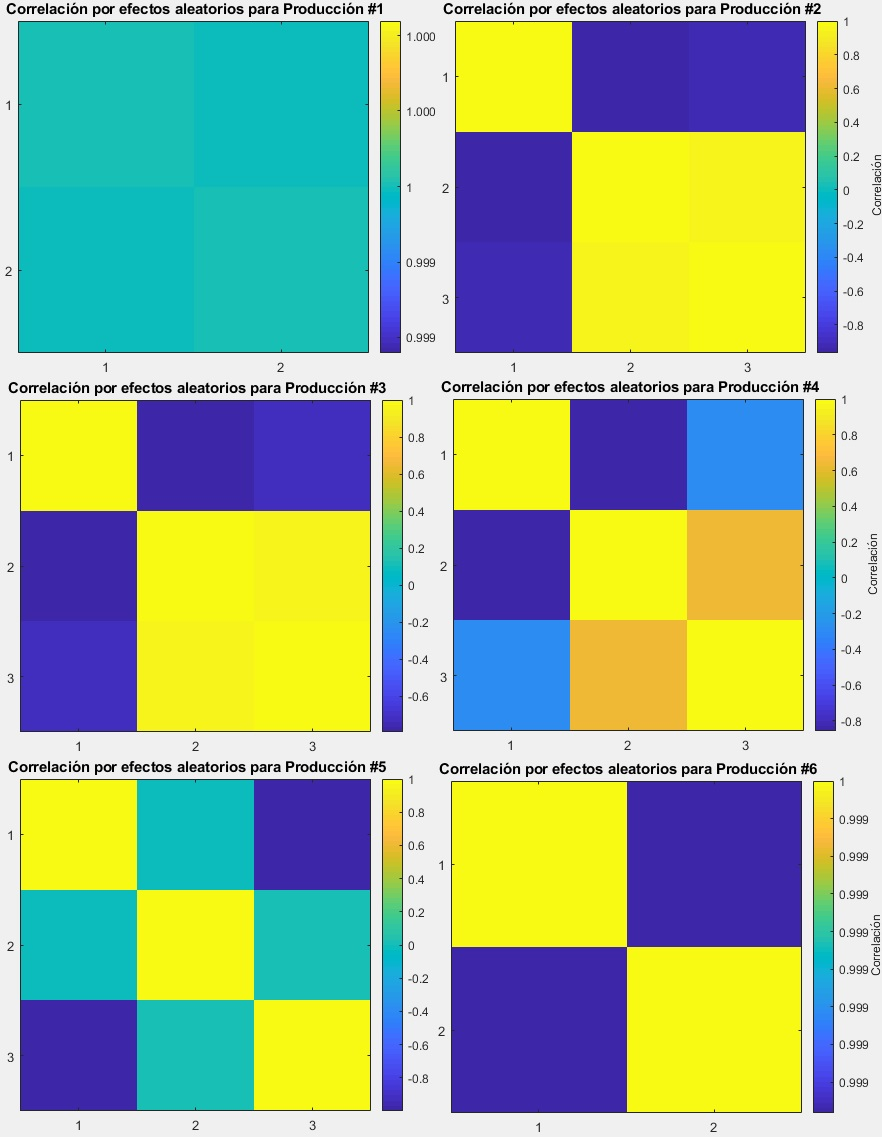
\includegraphics[scale=0.604]{img/covmatricesspa.jpg}
	 \end{center}
	 \caption{Matrices de covarianza del método ``nlmefit''. \label{covmatricespng}}
\end{figure}

\section{Relación matemática entre los parámetros $k_{1}$, $k_{2}$, $k_{3}$ y $k_{4}$}\label{demostralabel}

Partiendo de las Ecuaciones Diferenciales Ordinarias de primer orden \ref{modwp1} y \ref{modwp2} y considerando que estas ecuaciones estan relacionadas entre sí, se puede establecer una EDO de segundo orden que permita expresar una varible en función de otra de la siguiente manera:

% Por una parte sabemos que:
\begin{equation*}
    \frac{dW}{dt} = k_{1}\alpha_{s}W - k_{2}P, \hspace{0.6cm} \frac{dP}{dt} = k_{3}\alpha_{s}W - k_{4}P \hspace{0.2cm}, \hspace{0.3cm} \hspace{0.2cm} \frac{dW}{dt} = \dot{W}, \hspace{0.3cm} \frac{dP}{dt} = \dot{P}
\end{equation*}

% Reescribiendo P en terminos de W obteniendo W** 
% \begin{equation*}
%     \frac{dP}{dt} = k_{3}\alpha_{s}W - k_{4}P, \hspace{1cm} \frac{dP}{dt} = \dot{P}
% \end{equation*}

\begin{equation*}
    \ddot{W} = \frac{d}{dt}\left(\frac{dW}{dt}\right) \longrightarrow \ddot{W} = k_{1}\alpha_{s}\frac{dW}{dt} - k_{2}\frac{dP}{dt} \hspace{0.3cm} \longrightarrow \hspace{0.3cm} \ddot{W} = k_{1}\alpha_{s}\dot{W} - k_{2}\dot{P}\hspace{0.15cm}
\end{equation*}

Sabemos que el valor de $\dot{P}$, por lo que reemplazando en $\ddot{W}$ se obtiene:
\begin{equation*}
    \dot{P} = k_{3}\alpha_{s}W - k_{4}P, \hspace{0.2cm}\longrightarrow\hspace{0.2cm} \ddot{W} = k_{1}\alpha_{s}\dot{W} - k_{2}(k_{3}\alpha_{s}W - k_{4}P)
\end{equation*}

% Abrimos parentésis y reescribimos = 0
Separando las variables hacia los lados:
\begin{equation}
    \ddot{W}- k_{1}\alpha_{s}\dot{W} + k_{2}k_{3}\alpha_{s}W = k_{2}k_{4}P
\end{equation}

% suponiendo que k_{2}k_{4}P=0 y cambio de variable
Supóngase  $k_{2}k_{4}P\approx 0$, despejamos $\ddot{W}$, hacemos cambio de variable y resolvemos para $m = \ddot{W}$

% suponiendo que k_{2}k_{4}P=0 y cambio de variable
\begin{equation}
    % (a)m^{2} + (b)m + (c) = 0, \longrightarrow m=\frac{-b \pm \sqrt{b^{2}-4(a)(c)}}{2(a)} 
    % \longrightarrow
    m=\left(\frac{-b}{2a}\right) \pm \sqrt{\left(\frac{b}{2a}\right)^{2}-(c)} \hspace{0.2cm}
\end{equation}
Donde $\left[\left(\frac{b}{2a}\right)^{2} - (c)\right]$ decidirá el comportamiento amortiguado del sistema. Reemplazamos valores:
% Reescribimos la cuadrática y vemos la raíz
\begin{equation}
    m=\left[\left(\frac{k_{1}\alpha_{s}}{2}\right)\pm\sqrt{\left(\frac{k_{1}\alpha_{s}^{2}}{2}\right)-(k_{2}k_{3}\alpha_{s})} \hspace{0.2cm}\right] donde \hspace{0.2cm} \left(\frac{k_{1}\alpha_{s}}{2}\right)^{2}\geq k_{2}k_{3}\alpha_{s} 
\end{equation}

Despejando la desigualdad, y sabiendo de antemano que 
 $\alpha_{s}\neq 0$, se obtiene que:
\begin{equation} \label{relacionkis}
    \left(\frac{k_{1}\alpha_{s}}{2}\right)^{2}\geq k_{2}k_{3}\alpha_{s} \longrightarrow \left(\frac{k_{1}^{2}\alpha_{s}^{2}}{2^{2}}\right)\geq k_{2}k_{3}\alpha_{s} \longrightarrow k_{1}^{2}\geq 4\left(\frac{k_{2}k_{3}}{\alpha_{s}}\right)
\end{equation}
\subsection{Observaciones}
Basado en la representación por EDOs, tanto en las ecuaciones \ref{modwp1} y \ref{modwp2}, así como también por la representación gráfica del modelo, es importante mencionar que, $k_{2}$ debería ser igual a $k_{3}\alpha$, pues parte del peso que no se gana se debe a la producción de producto P que es expulsado del cuerpo del animal, ya sea por la producción de leche L en el proceso de ordeño o por producción de estiércol en el proceso de excreción de las necesidades biológicas del animal. \\

Por otra parte, el factor $k_{2}k_{4}P$ que se supone aproximadamente igual a 0, puede afectar el comportamiento final del sistema puesto que este valor únicamente sería 0 si el bovino no tuviera perdidas en la producción de desechos.

\section{Representación gráfica del modelo EDO-WP}\label{grafolabel}

\begin{figure}[H]
	 \begin{center}
	 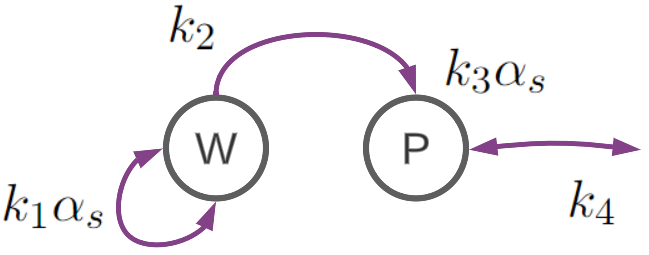
\includegraphics[scale=0.48504]{img/grafoedo.png}
	 \end{center}
	 \caption{Representación gráfica de las ecuaciones \ref{modwp1} y \ref{modwp2}. \label{anexografoedo}}
\end{figure}






